\documentclass[11pt,fleqn]{article} % Tipo de documento y tamaño. fleqn alinea las ecuaciones a la izquierda
%\ProvidesPackage{MyConfig}

\usepackage[utf8]{inputenc}% Caracteres especiales
\usepackage[T1]{fontenc}
\usepackage[spanish]{babel} % Idioma del documento
\usepackage[letterpaper,top=1.5cm,bottom=2cm,left=1.5cm,right=1.5cm]{geometry} % Márgenes
\usepackage{graphicx} % Para insertar imágenes
\usepackage{float} % Permite posicionar mejor las figuras y tablas
\usepackage{ragged2e} % Para centrar y justificar
\usepackage{url} % Para poner URL 
\usepackage{enumerate} % Modificar las enumeraciones
\usepackage{multirow} % Para unir columnas y filas
\usepackage{colortbl} % Color a las celdas de las tablas
\usepackage[dvipsnames]{xcolor} % Poder definir colores. El [dvipsnames] agreaga nombres de colores
\usepackage{longtable} % Para hacer tablas largas
\usepackage{tabularx} % Para hacer tablas que completen el largo de la página
\usepackage{array} % Según la wiki de tabular x, este paquete es necesario para que tabularx funcione bien. Además, agrega nuevas opciones a tabular
%\usepackage{slashbox,pict2e} % Para dar un slash en las tablas. pict2e mejora la línea
\usepackage{lmodern} % Cambia la fuente a una fuente vectorial, para que no haya problemas al reescalado
\usepackage{cancel} % Poder cancelar en las ecuaciones matemáticas
\usepackage{setspace} % Para establecer el interlineado
\usepackage{amsmath} % Mejora la escritura matemática
\usepackage{amsthm} % Ayuda a definir estructuras similares a teoremas
\usepackage{amssymb} % Añade símbolos matemáticos extra
\usepackage{titlesec} % Modificar los estidos de las secciones, subsecciones y subsubsecciones
\usepackage{multicol} % Añade distribución para hacer que todo el documento pueda ser a dos columnas.
\usepackage{caption} % Modifica el estilo del caption
\usepackage[hidelinks, breaklinks=true]{hyperref} % Linkear las citas y los urls. Hidelinks elimina los cuadros que se hacen a los lados. breaklinks=true se usa para que separe en líneas lo títulos muy largos
\usepackage{booktabs} % Nuevas líenas para hacer tablas

%%%%%%%%%%%%%%%%%%%%%%%%%%%%%%%%%%%%% Modificación secciones

\titleformat{\section}[block]{\normalfont \large \bfseries \color{BlueViolet}}{\arabic{section}.}{4pt}{} % Da formato a \section
\titlespacing{\section}{0cm}{16pt}{10pt} % Espacios de las secciones. El primero indica el espacio entre el borde del documento y el número. El segundo el espacio con el párrafo de arriba y el tercero el espacio con el párrafo de abajo

\titleformat{\subsection}[block]{\normalfont \large \itshape \color{BlueViolet}}{\arabic{section}.\arabic{subsection}.}{4pt}{}
\titlespacing{\subsection}{0cm}{16pt}{10pt}

\titleformat*{\subparagraph}{\normalfont \normalsize \itshape \color{BlueViolet}}

%%%%%%%%%%%%%%%%%%%%%%%%%%%%%%%%%%%%% Modificación caption

\captionsetup{font=small,justification=raggedright,singlelinecheck=false} % Modifica el estilo de los caption
\captionsetup[figure]{name={Fig.},labelsep=period,labelfont={bf,it,color=BlueViolet},textfont=it} % Modifica el nombre de las figuras y su separador
\captionsetup[table]{name={Tabla},labelsep=newline,labelfont={bf,color=BlueViolet}} % Modifica el nombre de las figuras y su separador

%%%%%%%%%%%%%%%%%%%%%%%%%%%%%%%%%%%%% Entornos tablas

%\renewcommand\tabularxcolumn[1]{>{\Centering}p{#1}} % Hace que el X de tabularx ahora esté centrado y no alineado a la izquierda
\newcolumntype{Y}{>{\raggedright\arraybackslash}X} % Crea el tipo Y que es como el X pero alineado a la izquierda

%%%%%%%%%%%%%%%%%%%%%%%%%%%%%%%%%%%%% Nuevos comandos

%\newcommand{\R}[1][2]{\mathbb{R}^{#1}} % Comando para espeficifar espacios dimencionales
\newcommand{\Cels}{$^{\circ}\text{C}$ } % Comando para escribir el símbolo de Celsius

%%%%%%%%%%%%%%%%%%%%%%%%%%%%%%%%%%%%% % Cargar configuración de otro archivo

\begin{document}
	\onehalfspacing % Modifica el interlineado
	\setlength{\parskip}{0cm} % Define el espacio entre párrafos
	\setlength{\parindent}{0cm} % Define la sangría de los párrafos
	\urlstyle{same} % Define la fuente para los URL de la bibliografía	
	
	\begin{small}
		\begin{tabularx}{\textwidth}{Y r}
			\multirow{3}{*}{
\includegraphics[scale=0.25]{Imagenes/Logo.png}} 
			& \\
			& \large \textcolor{Micolor}{Nombre materia} \\
			& 
		\end{tabularx}
	\end{small}
	
	\begin{flushleft}
		\textcolor{Micolor}{\Large \textbf{Nombre del documento}}
	\end{flushleft}

	Nombre1$^{\dag}$$^{a}$ y Nombre2$^{\dag}$$^{b}$
	
	\begin{small}
		\textit{$^{\dag}$Departamento de Química, Facultad de Ciencias, Universidad de los Andes, Carrera 1 N° 18 A 12, Bogotá, 111711, Colombia.}
		
		\textit{$^{a}$ correo1, $^{b}$ correo2}
		
		\linhor % Hace una línea horizontal
		
		\textcolor{Micolor}{\textbf{Resumen:}} Lorem Ipsum is simply dummy text of the printing and typesetting industry. Lorem Ipsum has been the industry's standard dummy text ever since the 1500s, when an unknown printer took a galley of type and scrambled it to make a type specimen book.  
	
		\textcolor{Micolor}{\textbf{Palabras clave:}} \textit{Palabra 1, palabra 2, palabra 3}
		
		\linhor
	\end{small}
	
	\setlength{\columnsep}{0.63cm} % Establece el espacio entre columnas
	
	%\begin{multicols*}{2} % El asterisco sirve para invalidar el balanceo de párrafos al final del documento
	\begin{multicols}{2}
%		\setlength{\parskip}{\baselineskip} % Define el espacio entre párrafos
		\setlength{\parindent}{0.5cm} % Define la sangría de los párrafos
				
		\section{Introducción} 
		
		\subsection{Subsección}
		
		\subparagraph{Sub Subsección}Lorem Ipsum is simply dummy text of the printing and typesetting industry. Lorem Ipsum has been the industry's standard dummy text ever since the 1500s, when an unknown printer took a galley of type and scrambled it to make a type specimen book. \cite{article}, \cite{1}, \cite{book}. 
				
		\subsection{Subsección}
		
		\begin{table}[H]
			\centering
			\caption{Tabla de ejemplo}
			\label{Tabla_1}
			\begin{tabularx}{0.5\textwidth}{X X X} 
				\toprule % Línea de más arriba
				\multicolumn{2}{c}{Item} & \\ 
				\cmidrule(r){1-2} % Línea no continua en la mitad
				Animal & Description & Price (\$)\\ 
				\midrule % Línea de la mitad
				Gnat & per gram & 13.65 \\
				& each & 0.01 \\
				Gnu & stuffed & 92.50 \\
				Emu & stuffed & 33.33 \\
				Armadillo & frozen & 8.99 \\ 
				\bottomrule % Línea final
			\end{tabularx}			
		\end{table}
		
		\section{Sección Experimental} 
		
		Imagen \ref{Montaje_exp}, esquema \ref{Esquema_1} y tabla \ref{Tabla_1}.
		
		\linhor % Hace una línea horizontal
		\begin{imagen}
			\centering
			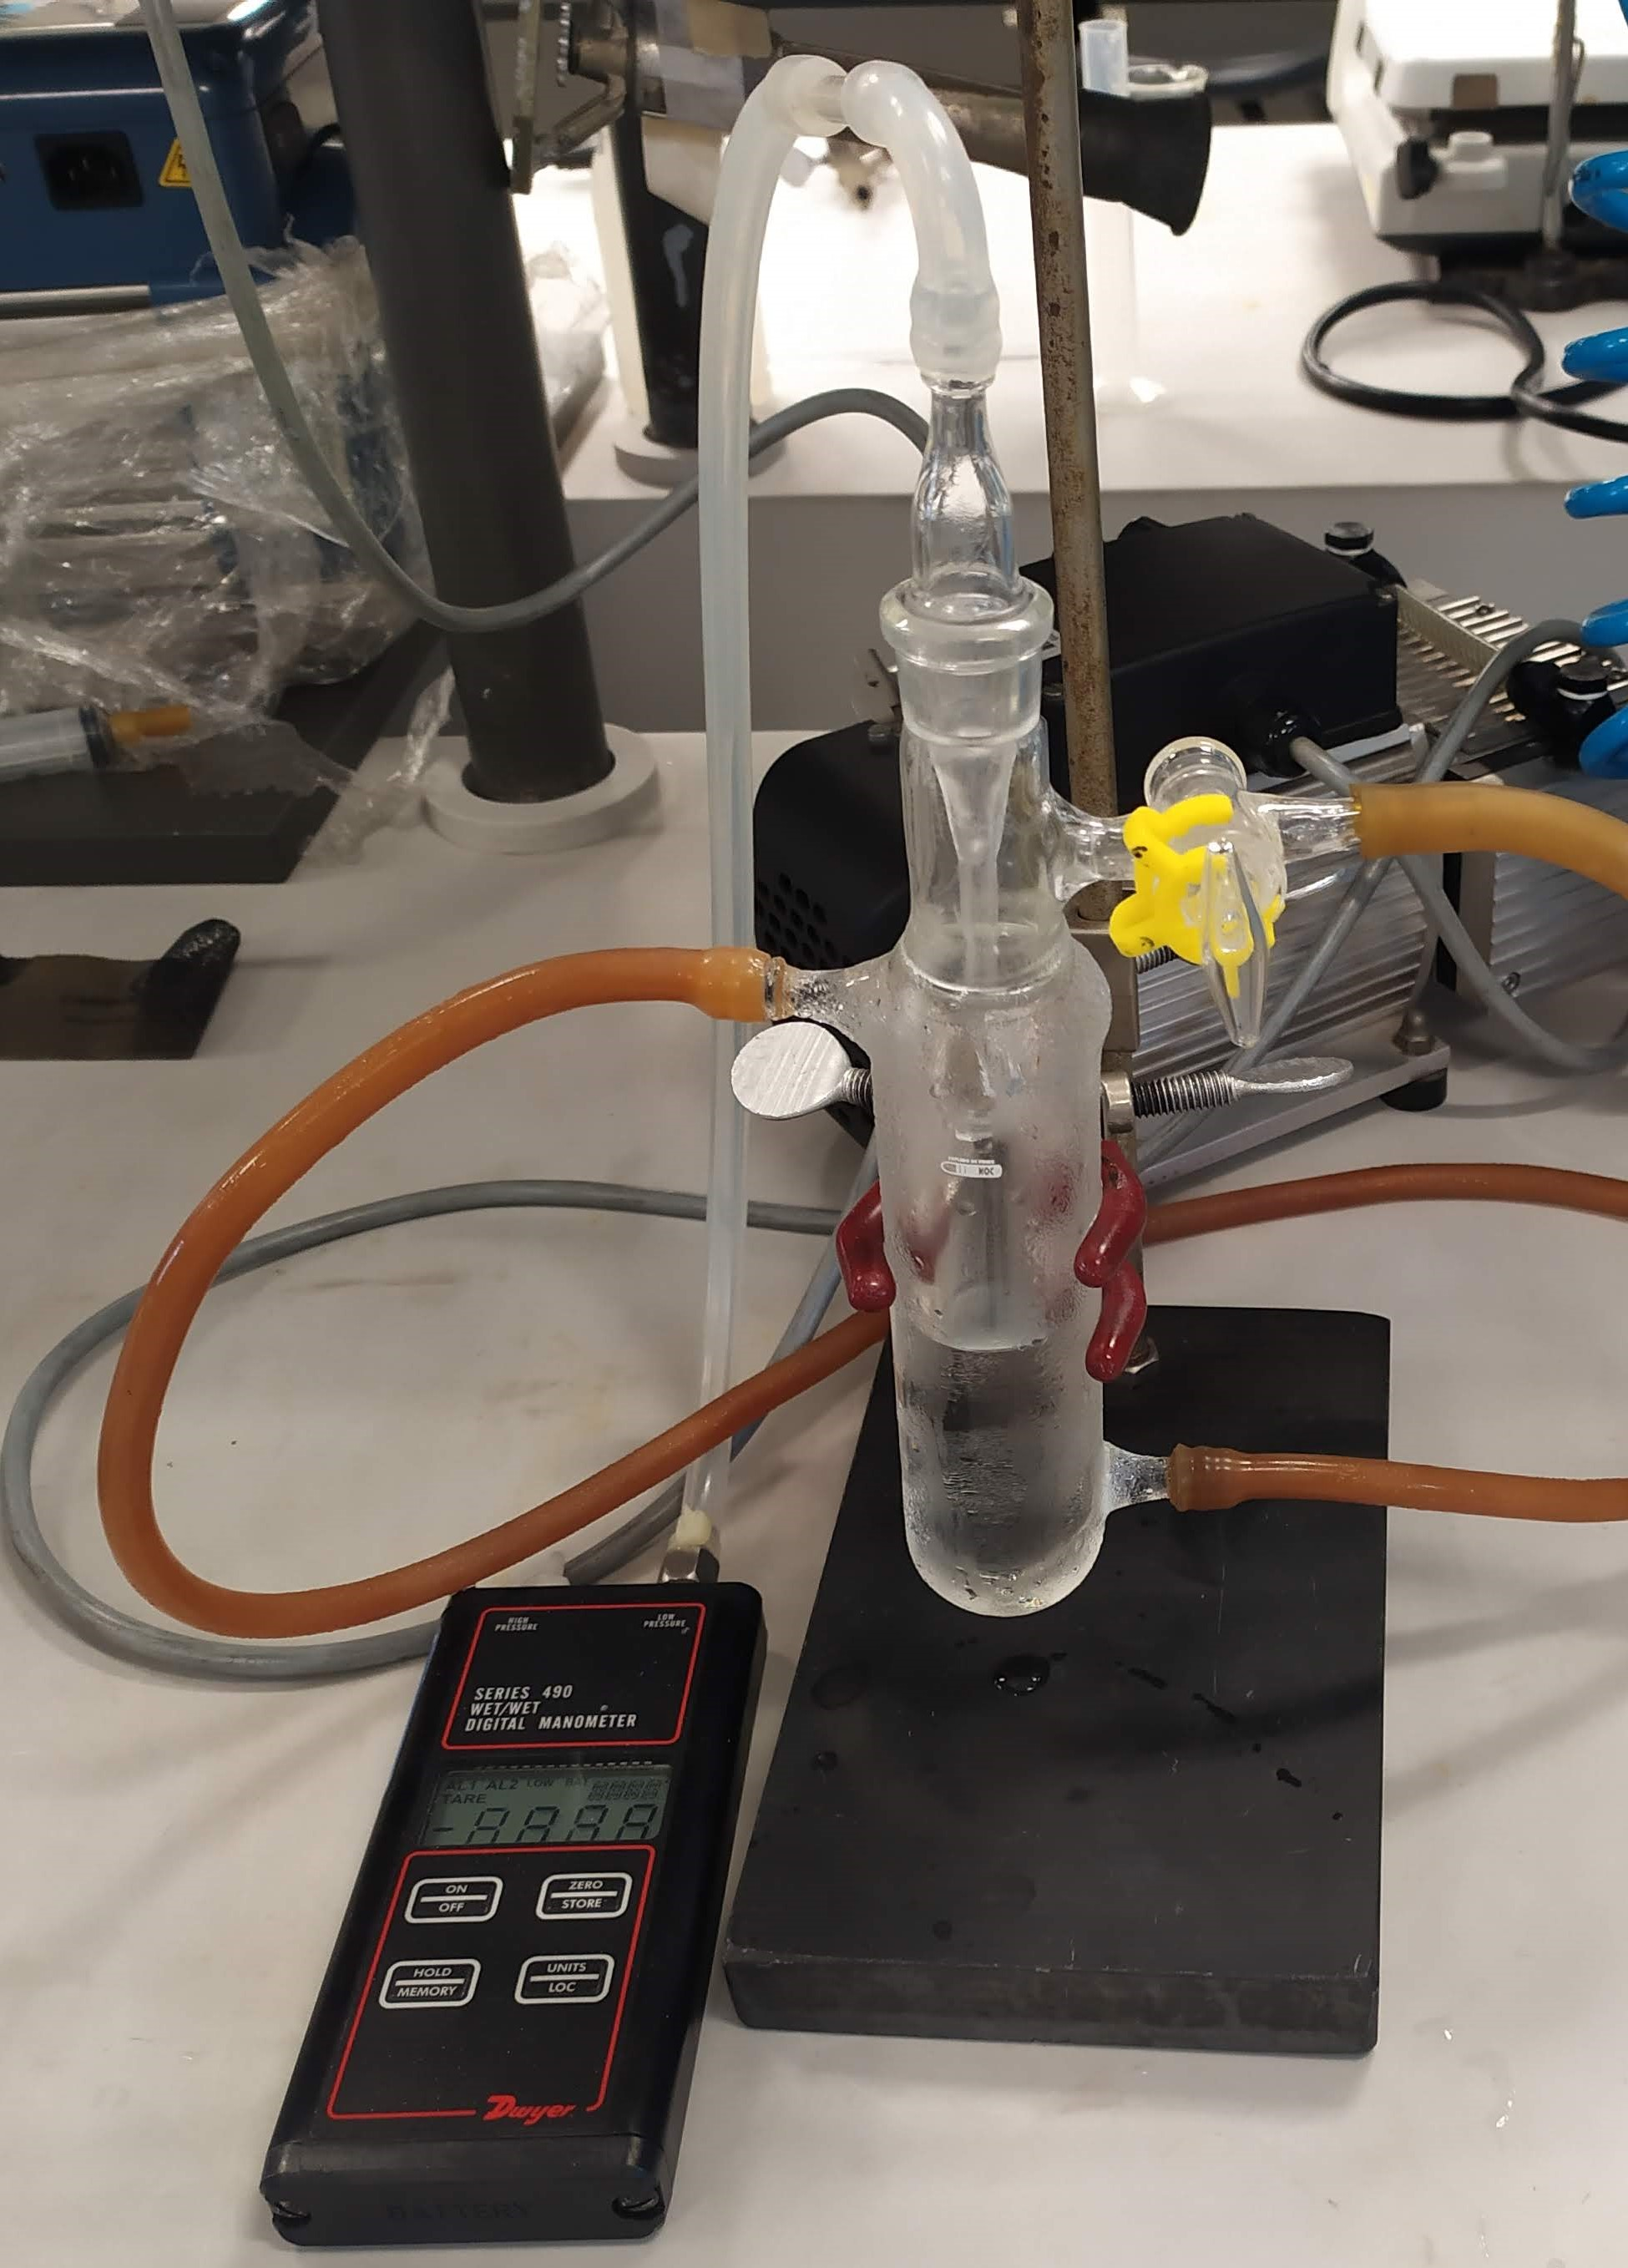
\includegraphics[scale=0.05]{Imagenes/Montaje.png}
			\caption{Montaje experimental} 
			\label{Montaje_exp}	
			\linhor
		\end{imagen}
		
		\linhor 
		\begin{esquema}
			\centering
			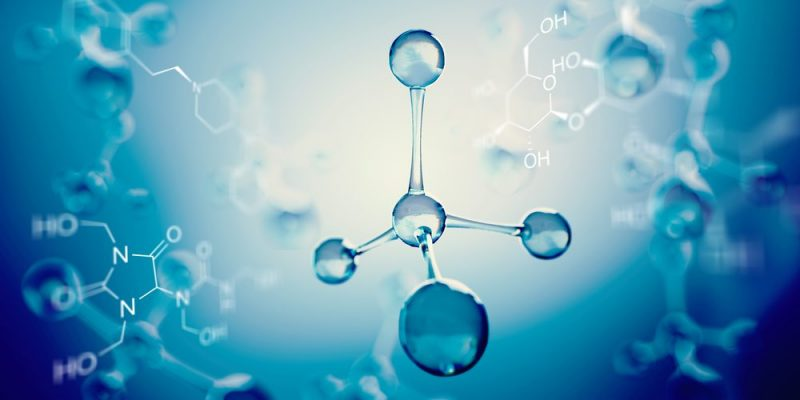
\includegraphics[scale=0.2]{Imagenes/Esquema.jpg}
			\caption{Montaje experimental} 
			\label{Esquema_1}	
			\linhor
		\end{esquema}
				
		\section{Resultados y discusión}
				
		\section{Conclusiones} 	 
		 
		\bibliography{bib} % Archivo con la bibliografía
		\bibliographystyle{acs-bib} % Estilo de la bibliografía
		
	\end{multicols}	

	\newpage % Nueva página
	\section*{Anexos} % El asterisco no enumera la sección
		
	\begin{multicols}{2}
		
		\begin{gather}
			A=\varepsilon \cdot b \cdot c \\
			A_{\lambda_1}=\varepsilon _{cuma \; \lambda_1} \cdot b \cdot c _{cuma} + \varepsilon _{vaini \; \lambda_1} \cdot b \cdot c _{vaini} \\
			A_{\lambda_2}=\varepsilon _{cuma \; \lambda_2} \cdot b \cdot c _{cuma} + \varepsilon _{vaini \; \lambda_2} \cdot b \cdot c _{vaini} \\
			\frac{A_{\lambda_1} - \varepsilon _{cuma \; \lambda_1} \cdot b \cdot c _{cuma}}{\varepsilon _{vaini \; \lambda_1} \cdot b} =  c _{vaini} = \varphi  \\
			\frac{A_{\lambda_2}}{b}= \varepsilon _{cuma \; \lambda_2} \cdot c _{cuma} + \varepsilon _{vaini \; \lambda_2} \cdot \varphi
		\end{gather}
		
	\end{multicols}	
	
\end{document}